\documentclass[twocolumn,aps,prd,nofootinbib,natbib]{revtex4-2}

\usepackage[utf8]{inputenc}
\usepackage[T1]{fontenc}
\usepackage{graphicx}
\usepackage{amssymb}
\usepackage{amsmath}
\usepackage{xcolor}
\usepackage{hyperref}
\usepackage{textcase}
\graphicspath{{figures/}}

\hypersetup{
  colorlinks=true,
  linkcolor=blue,
  urlcolor=blue,
  citecolor=blue
}
\urlstyle{same}

\begin{document}

\title{\MakeTextUppercase{Collapse-on-Command of an Actively Supported Rotating
Wormhole: Horizon Formation and Gravitational-Wave Emission Without an Imposed
Quadrupole Kick}}

\author{\MakeTextUppercase{Nikita M. Shirokov}}
\email{shirokov.nm@phystech.edu}
\affiliation{\textit{Independent Researcher, Moscow, Russia}}
\date{\today}

\begin{abstract}
We evolve a rotating, actively supported wormhole in three-dimensional numerical
relativity. Constraint-solved initial data contain an exotic complex scalar
Q-torus with winding $m=1$; collapse is triggered by ramping its support to zero
over $t\in[8,10]$, without an imposed perturbation. The lapse reaches
$\min\alpha\simeq10^{-3}$, the conformal factor pinches, and a coordinate-sphere
trapped-surface proxy grows to $r_{\rm AH}\simeq9.2$. The proxy then shrinks while
the lapse recovers, indicating a phantom-matter rebound rather than a quiescent
black hole. A coherent $\ell=2$ curvature wave propagates at approximately the
speed of light and is overwhelmingly $m=0$, linking the radiation primarily to
the collapsing toroidal density rather than to a nonaxisymmetric spin mode.
The collapse, rebound, and burst reproduce for base spacings
$h\simeq0.667,0.5,0.4$. Richardson behavior is quantity-dependent: selected
geometric and momentum-constraint measures converge, whereas the Hamiltonian
maximum and waveform peak do not admit controlled extrapolation. A completed
$L=128$ run gives an independent intermediate-zone waveform check. The result is
an engineered dynamical experiment, not a stationary solution of the unforced
Einstein--Klein--Gordon system.
\end{abstract}

\maketitle

\section{Introduction}
Traversable wormholes require null-energy-condition (NEC) violation
~\cite{morris88}. Static Ellis--Bronnikov throats are dynamically unstable:
compressive perturbations collapse them, while rarefactive perturbations drive
expansion~\cite{ellis73,bronnikov73,shinkai02,gonzalez09}. We ask whether support
can be withdrawn from a rotating exotic throat in a controlled way and whether
the collapse radiates without an imposed quadrupolar kick.

The rotation is carried by a complex scalar Q-torus rather than prescribed
through an analytic rotating metric. An elliptic solve supplies
constraint-consistent geometry and extrinsic curvature; an external support
coupling holds the composite configuration temporarily and provides the trigger.
This construction isolates the response to support removal but explicitly
introduces a nonconservative source while support is active.

\begin{figure*}[tp]
\centering
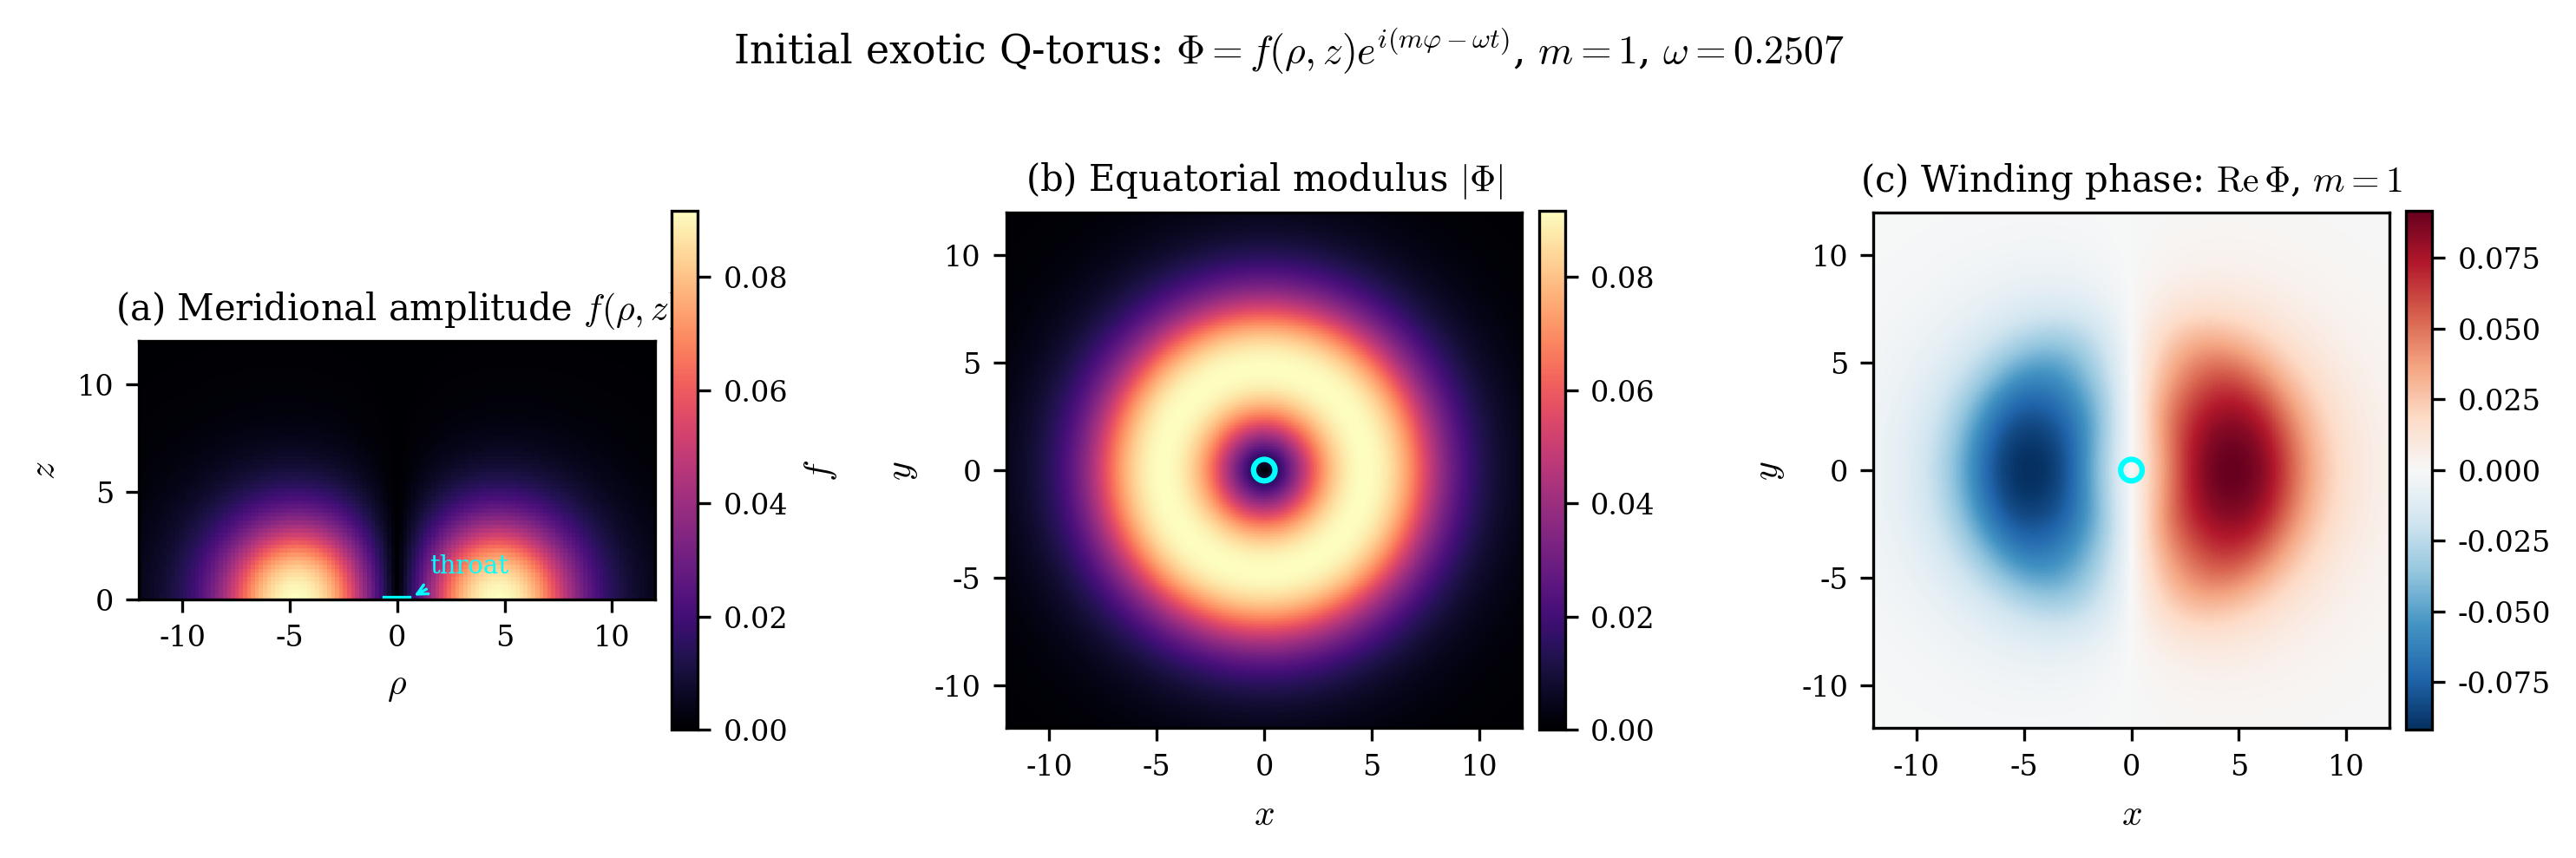
\includegraphics[width=0.98\textwidth]{fig_initial_matter.png}
\caption{Initial exotic matter. \textbf{(a)} The solved meridional eigenfunction
$f(\rho,z)$. \textbf{(b)} Its axisymmetric toroidal modulus on the equatorial
plane. \textbf{(c)} The real field at $t=0$, showing the $m=1$ phase winding.
The cyan circle/segment marks the throat scale. Thus the density is
axisymmetric although the complex phase carries angular momentum.}
\label{fig:initial_matter}
\end{figure*}

\section{Method}

\subsection{Evolution system and initial data}
We use the $3+1$ line element
\begin{equation}
 ds^2=-\alpha^2dt^2+\gamma_{ij}(dx^i+\beta^i dt)(dx^j+\beta^jdt)
\end{equation}
and evolve the CCZ4 system with \texttt{GRTeclyn}~\cite{grteclyn,grchombo}.
The conformal decomposition is
\begin{equation}
 \gamma_{ij}=\chi^{-1}\tilde\gamma_{ij},\qquad
 \det\tilde\gamma_{ij}=1 ,
\end{equation}
with $1+\log$ slicing and a Gamma-driver shift. A collapsing lapse diagnoses
strong gravitational collapse; $\chi\to0$ marks large metric stretching.

The seed slice is a puncture representation of an
Ellis--Bronnikov-class throat, not the analytic Teo metric~\cite{teo98}.
\texttt{GRTresna} solves the Hamiltonian and momentum constraints for the exact
throat-plus-matter configuration and exports a uniform \texttt{.gridinit} at the
evolution base spacing. The evolution is never initialized at finer spacing
than this solve.

The exotic complex scalar has potential
\begin{equation}
 V(|\Phi|^2)=\frac{\mu^2}{2}|\Phi|^2-\frac{\lambda}{4}|\Phi|^4
             +\frac{\mu_6}{6}|\Phi|^6
\end{equation}
with $\mu^2=0.5$, $\lambda=170$, and $\mu_6=1.445\times10^4$. Its stationary
flat-space profile is
\begin{equation}
 \Phi=f(\rho,z)e^{i(m\varphi-\omega t)},\qquad
 m=1,\quad\omega=0.2507 .
\end{equation}
The solved torus is shown in Fig.~\ref{fig:initial_matter}. Curvature and
self-gravity detune this profile after embedding, so the complete gravitating
object is actively supported rather than a passive equilibrium.

\subsection{Trigger and numerical setup}
The support strength is ramped from one to zero as
\begin{equation}
 S(t)=\frac{1}{2}\left[1+\cos\left(\pi\frac{t-8}{2}\right)\right],
 \qquad 8\le t\le10 ,
\end{equation}
with $S=0$ thereafter. No monopolar or quadrupolar field perturbation is added.

The headline domain has side $L=64$, base spacing $h=0.5$, and three AMR levels.
A sponge occupies $r=28$--$30$. The resolution ladder uses matched
\texttt{GRTresna} data at $h=0.667,0.5,0.4$, with otherwise identical evolution
parameters. The large-box check uses $L=128$, $h=0.5$, two AMR levels, a sponge
at $r=52$--$62$, and runs to $t=80$.

Because \texttt{GRTeclyn} has no production apparent-horizon finder, we use the
coordinate-sphere outgoing-expansion proxy
\begin{equation}
 \theta_+=\frac{2\sqrt{\chi}}{\bar r}
 -\frac{\partial_{\bar r}\chi}{\sqrt{\chi}}
 +\tilde A_{rr}-\frac{2}{3}K .
\end{equation}
The largest sampled radius with $\theta_+\le0$ defines $r_{\rm AH}$. This is a
trapped-surface indicator, not a horizon mass or spin measurement.

Surface integrals give $M_{\rm ADM}=0.209\pm0.001$ and
$J_{{\rm ADM},z}\simeq-1.93$ in code units. We do not use these values to make
precision detector forecasts because extraction systematics dominate.

\subsection{Wave extraction}
\label{sec:gw_extract}
We project $\Psi_4$ onto ${}_{-2}Y_{\ell m}$ on spheres at
$R_{\rm ext}=12,18,24$. Physics results use the post-processed Python extraction
from plotfiles; its files already store $r\Psi_4^{2,0}$. The in-code C++ Weyl
extraction is retained only for debugging because its $m=0$ imaginary component
fails the expected null test. In contrast, the Python signal has
$\max|\mathrm{Im}\Psi_4^{2,0}|/\max|\mathrm{Re}\Psi_4^{2,0}|\lesssim1.2\times10^{-3}$,
and more than $99.998\%$ of integrated $\ell=2$ power lies in $m=0$.

The headline radii are in the near zone. The $L=128$ run extracts at
$R_{\rm ext}=36,48$, both inside the sponge onset, and is therefore an
intermediate-zone check rather than a wave-zone extrapolation.

\section{Results}

\subsection{Collapse and rebound}
Once support vanishes, the lapse and conformal factor collapse while the
trapped-surface proxy grows (Fig.~\ref{fig:diagnostics}). In the headline run,
\[
 \min\alpha=9.8\times10^{-4},\quad
 \min\chi=0.0185,\quad
 \max r_{\rm AH}=9.18 .
\]
The robust proxy turns on after the support cut and peaks near $t=15.1$.
Thereafter $r_{\rm AH}$ shrinks to $1.92$ by $t=40$, while
$\min\alpha$ recovers to $0.033$. The longer $L=128$ run reaches comparable
collapse depth and loses the proxy by $t\simeq78.4$. We call this
collapse--rebound morphology a \emph{phantom bounce}; the term does not imply
that a true apparent horizon has been located.

\begin{figure}[htp]
\centering
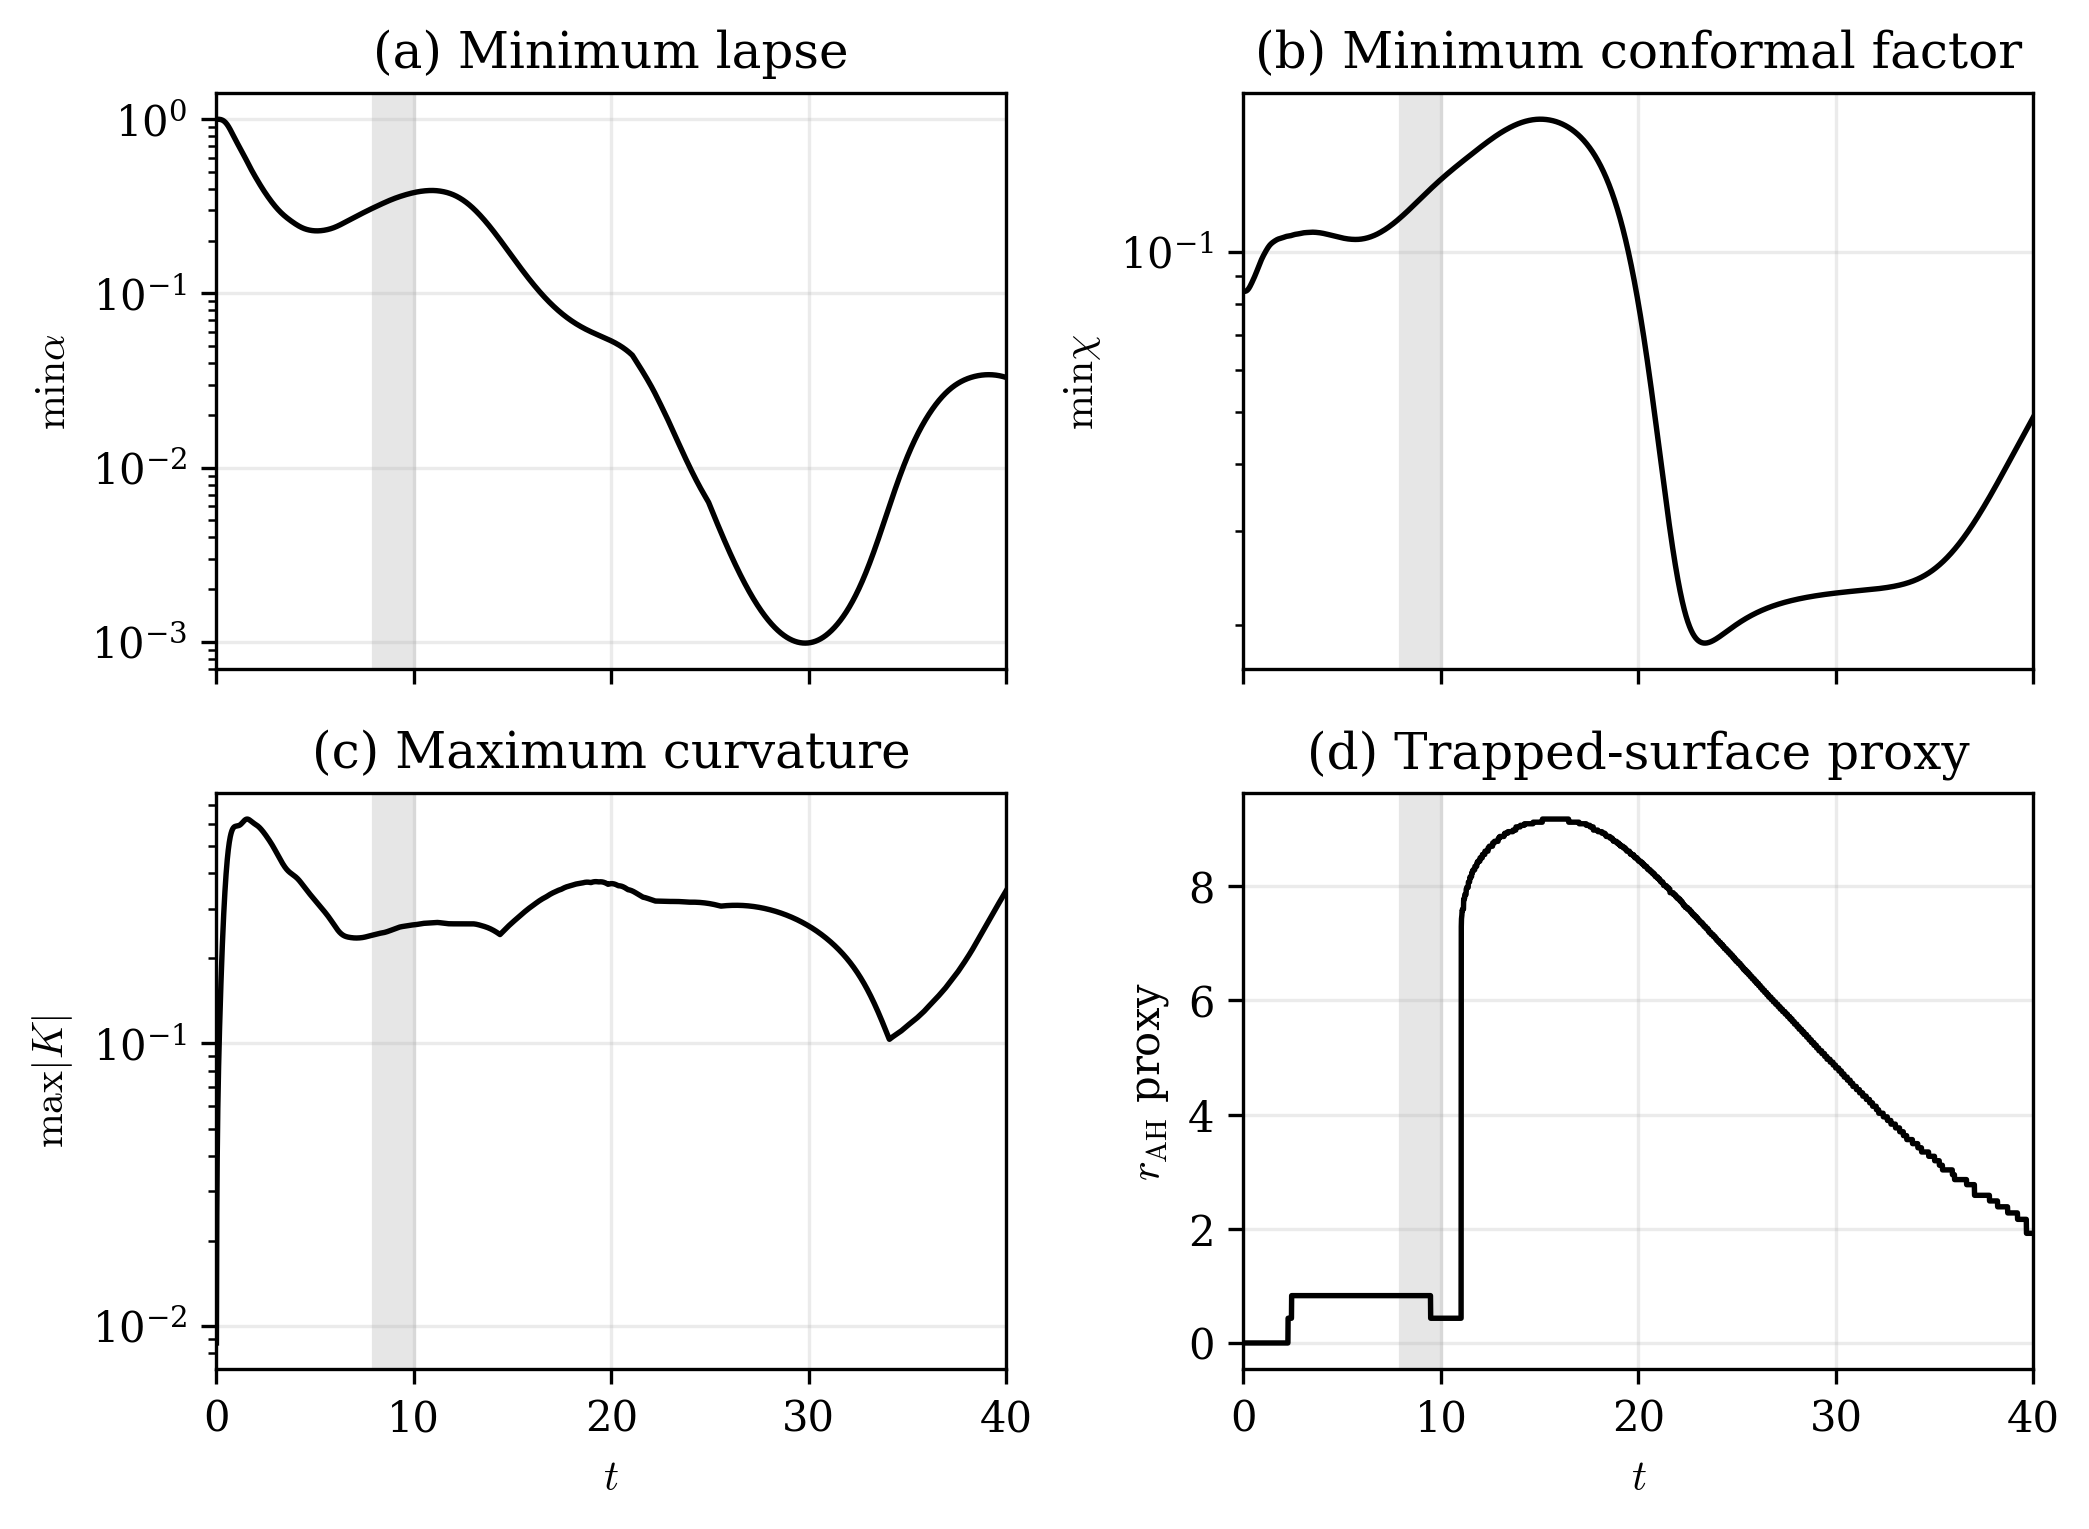
\includegraphics[width=\linewidth]{fig_collapse_diagnostics.png}
\caption{Headline collapse diagnostics. The support ramp is shaded. The lapse
and $\chi$ pinch as curvature grows; the trapped-surface proxy then forms and
subsequently shrinks.}
\label{fig:diagnostics}
\end{figure}

\subsection{Gravitational-wave signal}
The dominant $r\Psi_4^{2,0}$ signal is coherent across extraction radii and its
peak delay is consistent with propagation at $c$ to the post-processing cadence.
Its $m=0$ dominance means that the principal quadrupole follows the changing
toroidal density; it is not evidence for an $m=2$ bar mode.

Figure~\ref{fig:wave_systematics}(a) compares the three resolutions at $R=12$.
The medium and fine curves closely agree, but the coarse post-processing record
has no samples over part of the principal burst. We therefore do not assign a
three-point Richardson order to the burst amplitude. In the large box,
$R=36$ and $R=48$ align in retarded time with overlap $0.993$ after a residual
shift of $0.35$ and a relative $L_2$ residual of $12.3\%$
[Fig.~\ref{fig:wave_systematics}(b)]. This supports approximate $1/r$ behavior
in the intermediate zone. Late growth at $R=36$ is not shared by $R=48$ and
coincides with constraint growth, so it is not interpreted as a runaway
gravitational-wave instability.

\begin{figure*}[tp]
\centering
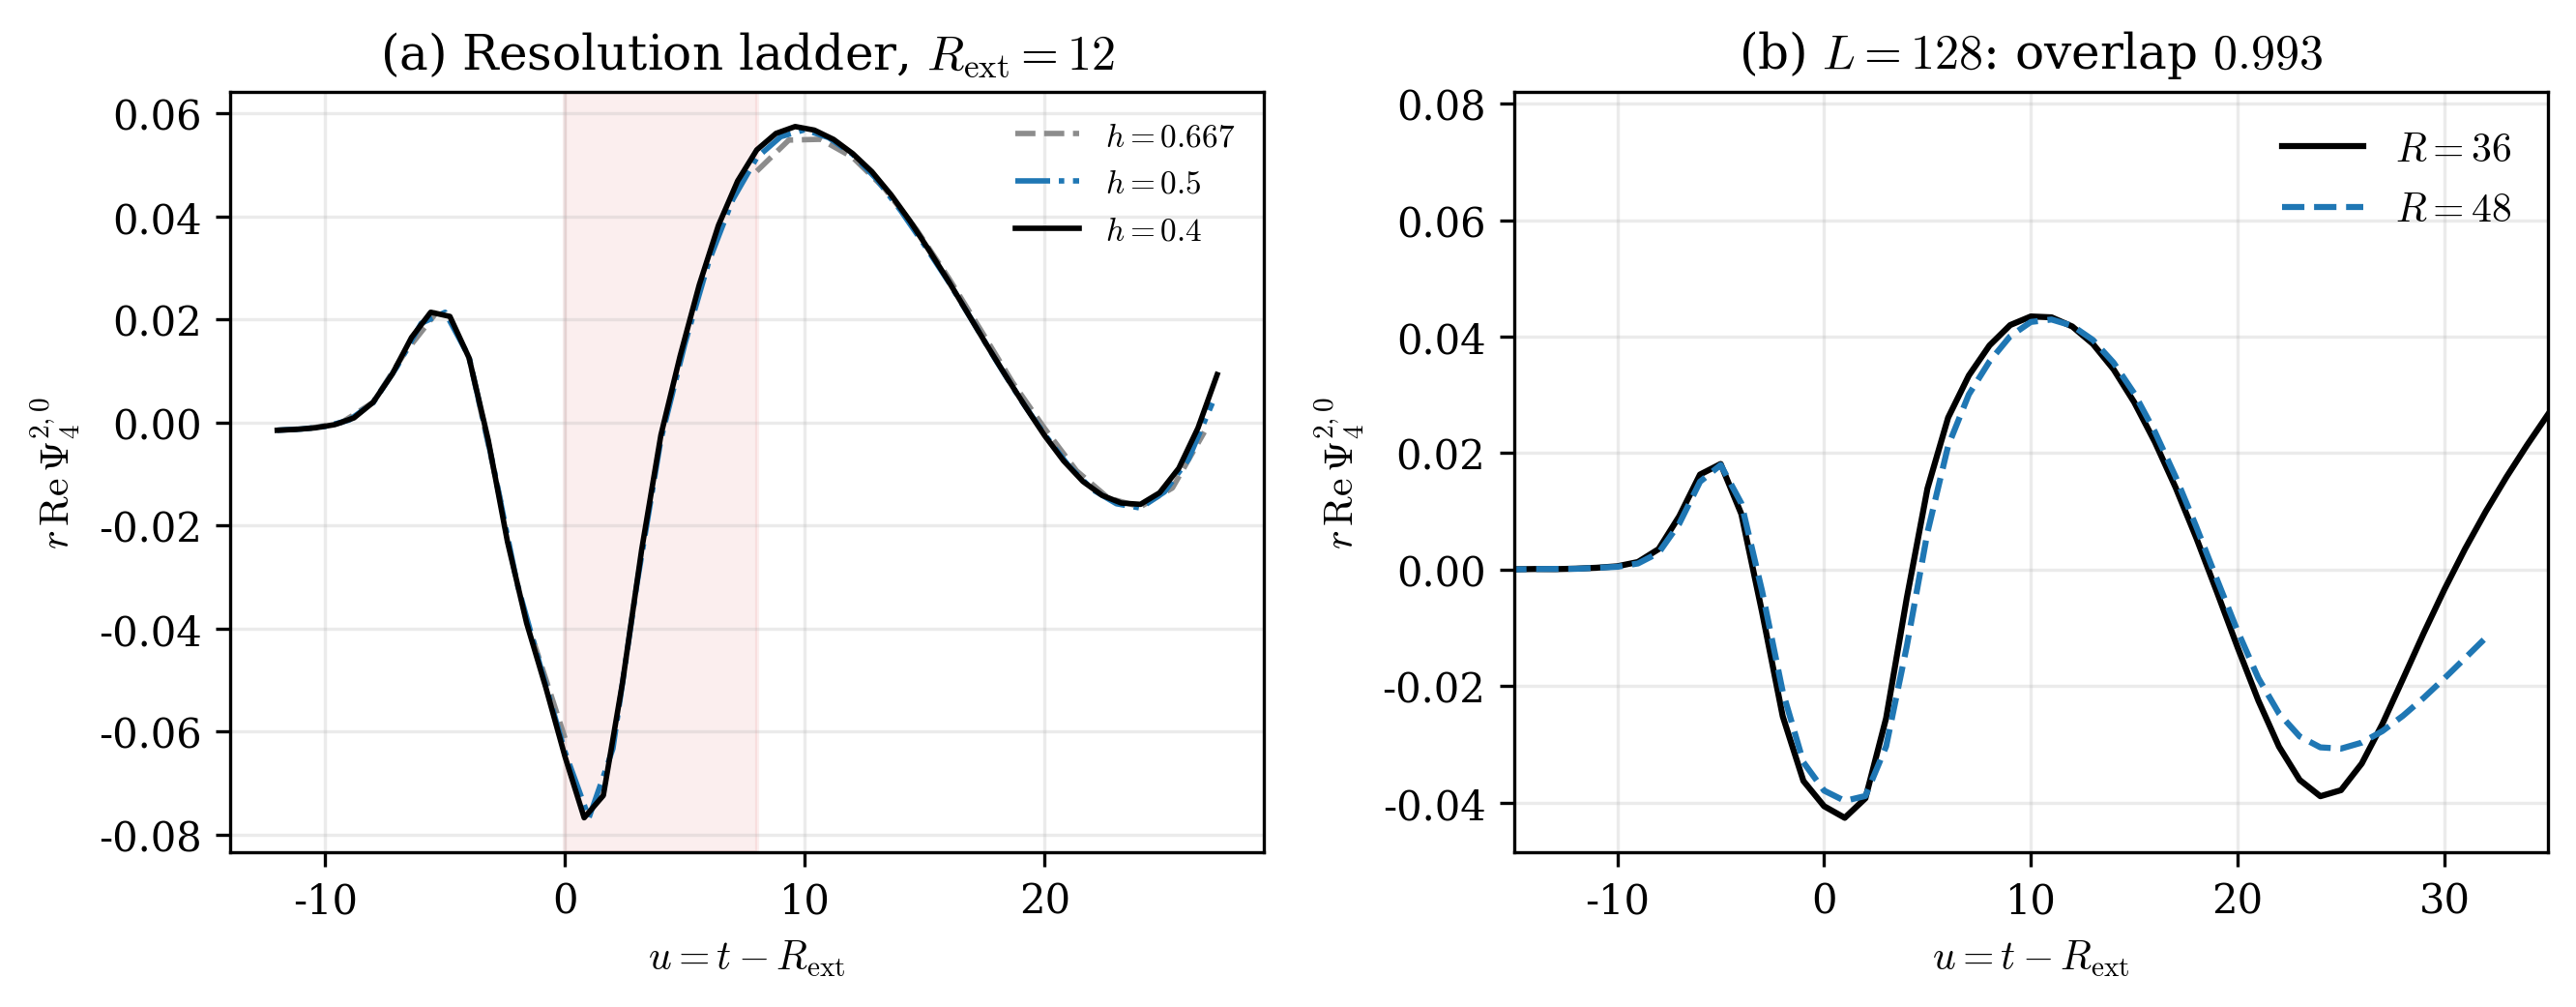
\includegraphics[width=0.94\textwidth]{fig_waveform_systematics.png}
\caption{\textbf{(a)} Validated $r\Psi_4^{2,0}$ at $R_{\rm ext}=12$ for the
resolution ladder; the shaded region includes the coarse extraction gap and is
excluded from formal waveform convergence. \textbf{(b)} Retarded-time comparison
at $R=36,48$ in the $L=128$ run. The agreement is an intermediate-zone
cross-check, not a fourth resolution rung.}
\label{fig:wave_systematics}
\end{figure*}

\subsection{Constraints and controls}
For the headline run, the volume-weighted norms remain below
$\|\mathcal H\|_2=3.25\times10^{-2}$ and
$\|\mathcal M\|_2=9.67\times10^{-3}$ through $t=40$
(Fig.~\ref{fig:constraints}). The large-box norms are smaller than these values
through $t=40$ but later reach $0.155$ and $0.0417$, respectively. Consequently
its late waveform is treated cautiously.

\begin{figure}[htp]
\centering

\includegraphics[width=\linewidth]{fig_constraints.png}
\caption{Volume-weighted Hamiltonian and momentum constraint norms for the
$h=0.5$ headline run. They remain bounded through the collapse and emission
interval.}
\label{fig:constraints}
\end{figure}

No-ramp and delayed-ramp controls do not produce the same resolved deep-collapse
branch before numerical failure. A nonrotating run built from the same toroidal
modulus follows a pathological trajectory: its coordinate-sphere proxy expands,
momentum constraints grow rapidly, and AMR memory approaches exhaustion. It was
stopped at $t\simeq13.5$. Thus the present data do not isolate rotation from
toroidal geometry; the measured $m=0$ dominance only shows that rotation is not
radiated mainly through nonaxisymmetric $\ell=2$ modes.

\subsection{Resolution study}
\label{sec:convergence}
For unequal spacings we assume, only where supported,
\begin{equation}
 Q(h)=Q_0+Ch^p
\end{equation}
and solve
\begin{equation}
 \frac{Q_c-Q_m}{Q_m-Q_f}
 =\frac{h_c^p-h_m^p}{h_m^p-h_f^p}
\end{equation}
for $p>0$. Sign-changing differences or unphysical continuum estimates are
reported as non-asymptotic.

All three runs reproduce the collapse, peak proxy radius, shrinkage, lapse
recovery, and axisymmetric burst (Fig.~\ref{fig:convergence}). Selected scalar
measures admit formal orders:
\[
\begin{array}{lccc}
Q & p & Q_0 & {\rm GCI}_f\\
\hline
\max|K| & 3.78 & 0.663 & 3.31\%\\
\max r_{\rm AH} & 0.91 & 9.39 & 2.39\%\\
t(\max r_{\rm AH}) & 2.09 & 14.68 & 2.42\%\\
\max\|\mathcal M\|_2 & 1.82 & 9.45\times10^{-3} & 1.95\%
\end{array}
\]
The Hamiltonian maximum instead increases slightly,
$0.0310\to0.0325\to0.0340$, and has no positive observed order. The lapse and
$\chi$ minima deepen with refinement but extrapolate to unphysical negative
values under the one-term model. These quantities establish qualitative
multi-resolution robustness, not a universal continuum order.

\begin{figure*}[tp]
\centering
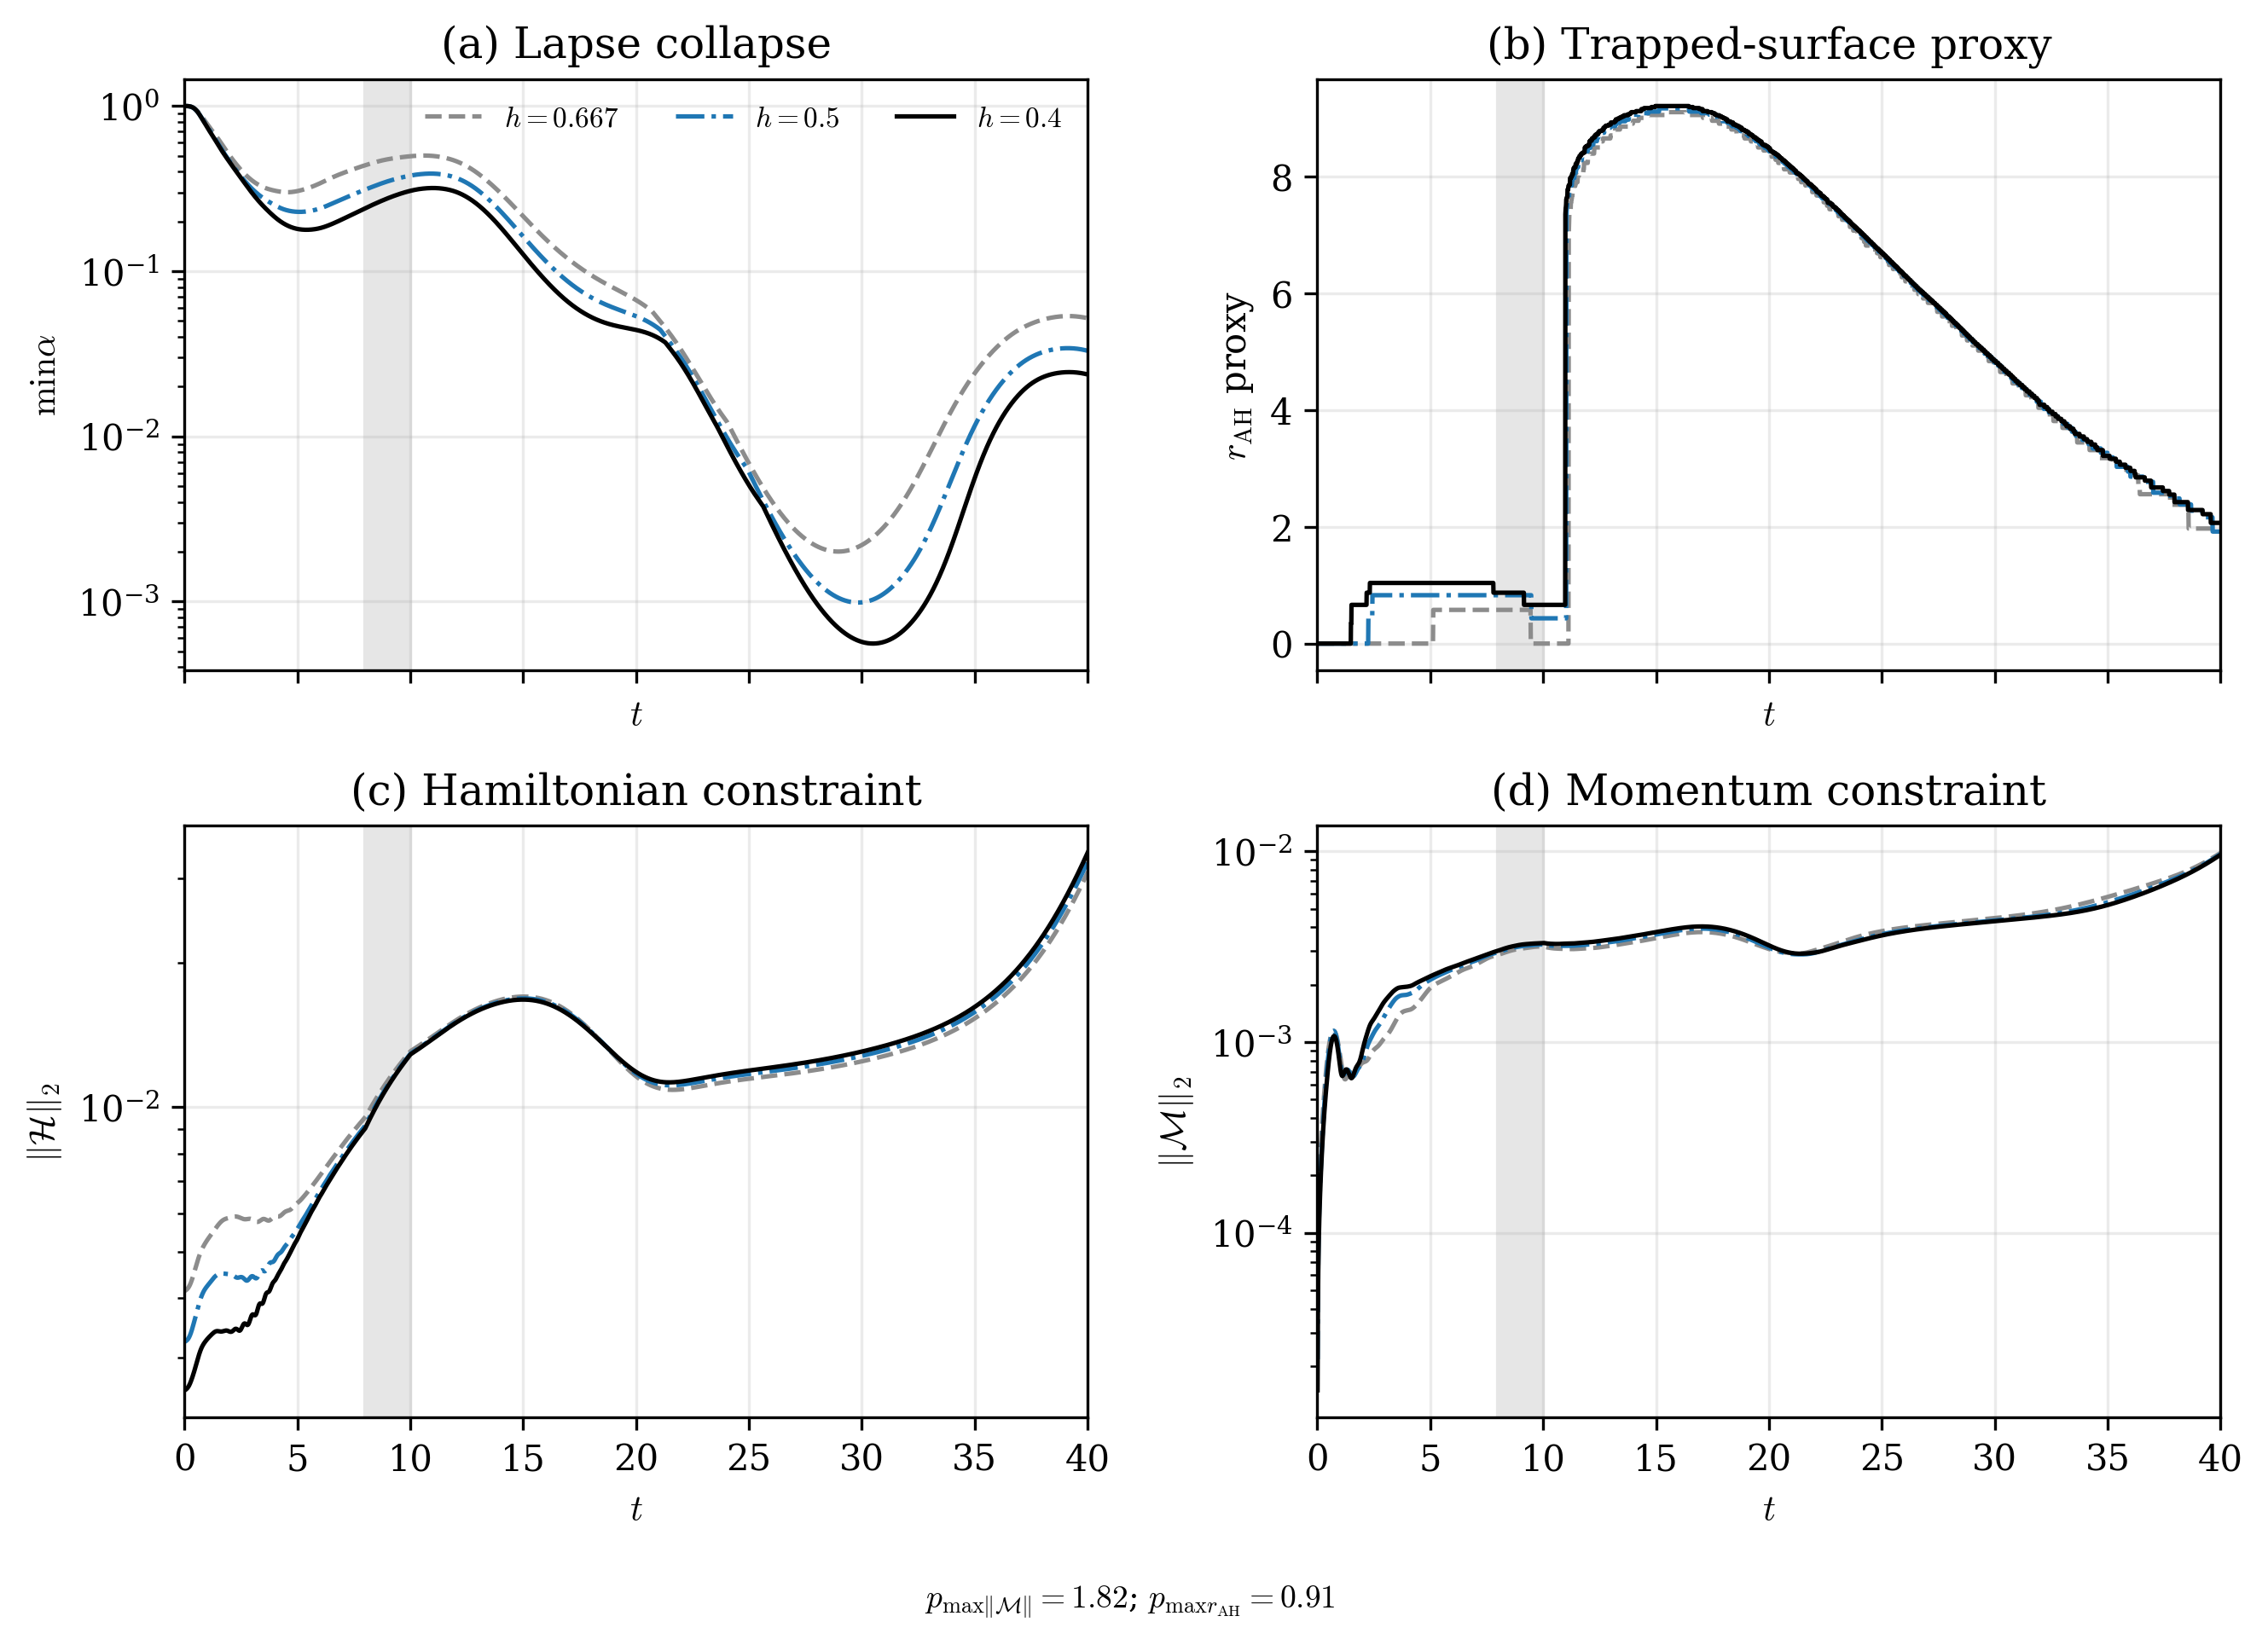
\includegraphics[width=0.92\textwidth]{fig_convergence.png}
\caption{Resolution ladder at $h=0.667,0.5,0.4$. The support ramp is shaded.
Collapse and proxy shrinkage are common to all runs. Momentum constraints show
limited convergence; Hamiltonian maxima remain bounded but do not converge
monotonically.}
\label{fig:convergence}
\end{figure*}

\section{Discussion}
Withdrawing support from this rotating exotic throat produces a trapped-surface
proxy, a collapsing lapse, and a coherent $\ell=2$ wave without an imposed kick.
The same collapse--rebound morphology appears at three resolutions and in a
larger domain. This removes the strongest single-resolution and small-box
concerns, but it does not turn every observable into a precision result.

Three limitations define the claim. First, $r_{\rm AH}$ is a coordinate-sphere
proxy; a production apparent-horizon finder is needed for horizon mass and spin.
Second, the waveform is extracted at finite, intermediate radii, and the coarse
record misses part of the main burst. Third, active support is an external,
nonconservative source, and whole-domain charge and angular momentum budgets do
not close. The result is therefore a controlled numerical experiment on an
engineered spacetime.

Future work should obtain a clean nonrotating control, add a genuine
apparent-horizon finder, repeat the large box at higher AMR depth, and use
wave-zone or characteristic extraction. These steps are required before quoting
precision energies, quasinormal frequencies, or detector horizons.

\section{Code and Data Availability}
The evolution example, initial-data solver, run parameters, validated
\texttt{small\_data/psi4\_mode\_l2m0.dat} files, diagnostics, and figure scripts
are maintained in the project repository. The manuscript directory contains
only the figures used here.

\section{Acknowledgements}
The author thanks Ilya Nachevsky for providing the high-performance computing
resources and acknowledges the GRTL collaboration for \texttt{GRChombo} and
\texttt{GRTeclyn}.

\begin{thebibliography}{99}
\bibitem{baumgarte10} T.~W.~Baumgarte and S.~L.~Shapiro,
\textit{Numerical Relativity: Solving Einstein's Equations on the Computer}
(Cambridge University Press, 2010).
\bibitem{morris88} M.~S.~Morris and K.~S.~Thorne,
\textit{Am.\ J.\ Phys.}\ \textbf{56}, 395 (1988).
\bibitem{kleihaus14} B.~Kleihaus and J.~Kunz,
\textit{Phys.\ Rev.\ D}\ \textbf{90}, 121503 (2014).
\bibitem{ellis73} H.~G.~Ellis, \textit{J.\ Math.\ Phys.}\ \textbf{14}, 104 (1973).
\bibitem{bronnikov73} K.~A.~Bronnikov, \textit{Acta Phys.\ Pol.\ B}\ \textbf{4},
251 (1973).
\bibitem{shinkai02} H.~Shinkai and S.~A.~Hayward,
\textit{Phys.\ Rev.\ D}\ \textbf{66}, 044005 (2002).
\bibitem{gonzalez09} J.~A.~Gonz\'alez, F.~S.~Guzm\'an, and O.~Sarbach,
\textit{Class.\ Quantum Grav.}\ \textbf{26}, 015010 (2009).
\bibitem{teo98} E.~Teo, \textit{Phys.\ Rev.\ D}\ \textbf{58}, 024014 (1998).
\bibitem{grteclyn} GRTL Collaboration, \texttt{GRTeclyn}: a GPU-accelerated,
AMReX-based numerical-relativity code,
\url{https://github.com/GRTLCollaboration/GRTeclyn}.
\bibitem{grchombo} T.~Andrade \textit{et al.},
\textit{J.\ Open Source Softw.}\ \textbf{6}, 3703 (2021).
\end{thebibliography}

\end{document}
